\documentclass[12pt,french]{article} %ajouter draft pour voir débordement
\usepackage[utf8]{inputenc}
\usepackage[T1]{fontenc}
\usepackage{lmodern}
%règles mes marges et format papier
\usepackage[a4paper,hmargin=2cm,vmargin=2cm]{geometry} %modif marge et formet
\usepackage{amsmath, amssymb, amsthm}
\usepackage{fancyhdr} %pour les entêtes et bas de page
\usepackage{lastpage} %pour numéroter les pages charge la derniere page
\usepackage{graphicx} %pour inclure des img
\usepackage{dsfont}
\usepackage{float} %pour le placement des figures
\usepackage{hyperref} %pour mettre des liens hypertext
\usepackage{calc} %permet de calculer les marges pour encadrer les textes
\usepackage{color, xcolor} %gère les couleurs
\usepackage{babel}
\usepackage{listings} %pour afficher le code annexe

%pour afficher le code de manière esthétique
\lstset{
  aboveskip=3mm,
  belowskip=-2mm,
  backgroundcolor=\color{white},
  basicstyle=\footnotesize,
  breakatwhitespace=false,
  breaklines=true,
  captionpos=b,
  commentstyle=\color{red},
  deletekeywords={...},
  escapeinside={\%*}{*)},
  extendedchars=true,
  framexleftmargin=16pt,
  framextopmargin=3pt,
  framexbottommargin=6pt,
  frame=tb,
  keepspaces=true,
  keywordstyle=\color{blue},
  language=C,
  literate=
  {²}{{\textsuperscript{2}}}1 {⁴}{{\textsuperscript{4}}}1
  {⁶}{{\textsuperscript{6}}}1
  {⁸}{{\textsuperscript{8}}}1
  {€}{{\euro{}}}1 {é}{{\'e}}1 {è}{{\`{e}}}1 {ê}{{\^{e}}}1 {ë}{{\¨{e}}}1
  {É}{{\'{E}}}1 {Ê}{{\^{E}}}1 {û}{{\^{u}}}1 {ù}{{\`{u}}}1 {â}{{\^{a}}}1
  {à}{{\`{a}}}1 {á}{{\'{a}}}1 {ã}{{\~{a}}}1 {Á}{{\'{A}}}1 {Â}{{\^{A}}}1
  {Ã}{{\~{A}}}1 {ç}{{\c{c}}}1 {Ç}{{\c{C}}}1 {õ}{{\~{o}}}1 {ó}{{\'{o}}}1 
  {ô}{{\^{o}}}1 {Õ}{{\~{O}}}1 {Ó}{{\'{O}}}1 {Ô}{{\^{O}}}1 {î}{{\^{i}}}1
  {Î}{{\^{I}}}1 {í}{{\'{i}}}1 {Í}{{\~{Í}}}1,
  morekeywords={*,...},
  numbers=left,
  numbersep=10pt,
  numberstyle=\tiny\color{black},
  rulecolor=\color{black},
  showspaces=false,
  showstringspaces=false,
  showtabs=false,
  stepnumber=1,
  stringstyle=\color{gray},
  tabsize=4,
}
%%%%%

%Personalisation En tête
\pagestyle{fancy}
\renewcommand\headrulewidth{1pt}
%permet d'aumenter tailler header pour mettre image (31pt ici)
\setlength{\headheight}{31pt} 
\fancyhead[L]{TP de SDD 1}
\fancyhead[C]{
\includegraphics[scale=0.05]{uca-p.png}}
\fancyhead[R]{2021/2022}
\renewcommand\footrulewidth{1pt}
\fancyfoot[L]{BALLEJOS Lilian}
\fancyfoot[C]{\thepage/\pageref{LastPage}}
\fancyfoot[R]{LEGER Bertrand}
%Fin personalisation En Tête


\begin{document}

\begin{titlepage} %page d'acceuil

  \begin{center}
  	
\includegraphics[scale=1.6]{gardeisima.png}
  \end{center}
  	
  \vspace*{2.5cm} %espace de 2.5cm en dessous des images
  
  \begin{center}\huge
    \textbf{Rendu TP : TP1 SDD} 
    
    \textbf{Agenda}
  \end{center}
  
  \hrule %trait horizontal
  
  \begin{center}
    \Large BALLEJOS Lilian
    
    \Large LEGER Bertrand
    
    \large Isima INP
    
    Année Universitaire 2021 - 2022
  \end{center}
  
  \begin{center}
    %créer une boite ou mettre l'image qui fait la largeur de la page
    \makebox[\textwidth]{
\includegraphics[width=\paperwidth]{garde.png}}
  \end{center}
  
  \vspace*{2cm} 
  
  \begin{flushright}\footnotesize %a droite
    Enseignant TP: CROMBEZ Loic
    
    Date du rendu: 7 mars 2022
    
    
  \end{flushright}
  
  \begin{flushleft}\small %a gauche
    \textbf{INP ISIMA}
    \footnotesize
    
    1 Rue de la Chebarde, 63178 Aubière
    
    Tel: 04 73 40 50 00
    
    Site web: \href{https://www.isima.fr/}{isima.fr}\newline 	
  \end{flushleft}
\end{titlepage}	

%Ma table des Matières !
%permet de renommer 'table des matières' en sommaire
\renewcommand{\contentsname}{Sommaire}
\normalsize\tableofcontents %place la table des matières

\vspace{0.5cm}

\section{Présentation du TP}

Ce TP a pour but d'implémenter une liste simplement chainée qui représente un pseudo Agenda. Nous avons ici séparé notre structure de donnée en 3 sous structures:\newline

\begin{itemize}
	\item La structure \textbf{"tête"} qui est la tête fictive qui pointe sur la première semaine,
	\item La structure \textbf{"semaine"} qui contient un numéro de semaine,une année (toutes concaténées dans la même chaine de caractère), un pointeur sur la semaine suivante ainsi qu'un pointeur sur la liste des actions qui ont lieu cette semaine,
	\item La structure \textbf{"action"} qui possède un numéro correspondant à un jour de la semaine, une heure (le tout concaténées dans la même chaine de caractère), le nom de l'action et enfin un pointeur vers l'action suivante.\newline
\end{itemize}

Nous avons créé un fichier source $".c"$ par structure (tete.c, action.c, semaine.c), un fichier "commun.c" qui contient toutes les fonctions en lien avec l'ensemble des 3 structures et enfin un fichier main.c qui contient le main. 
\newline

Tous les fichiers sources sont stockés dans le dossier "source", les fichiers "headers" dans le dossier header, les fichiers objets dans le dossier "objet" et enfin les entrées et sorties de notre programme dans les dossiers "entree" et "sauvegarde".
Un makefile est fourni pour tout compiler et génére l'executable \textbf{"Programme"}.

\section{Présentation de la structure}
\subsection{Schéma de la structure}

Voici un schéma de la structure que nous avons mis en place :

\begin{figure}[H]
	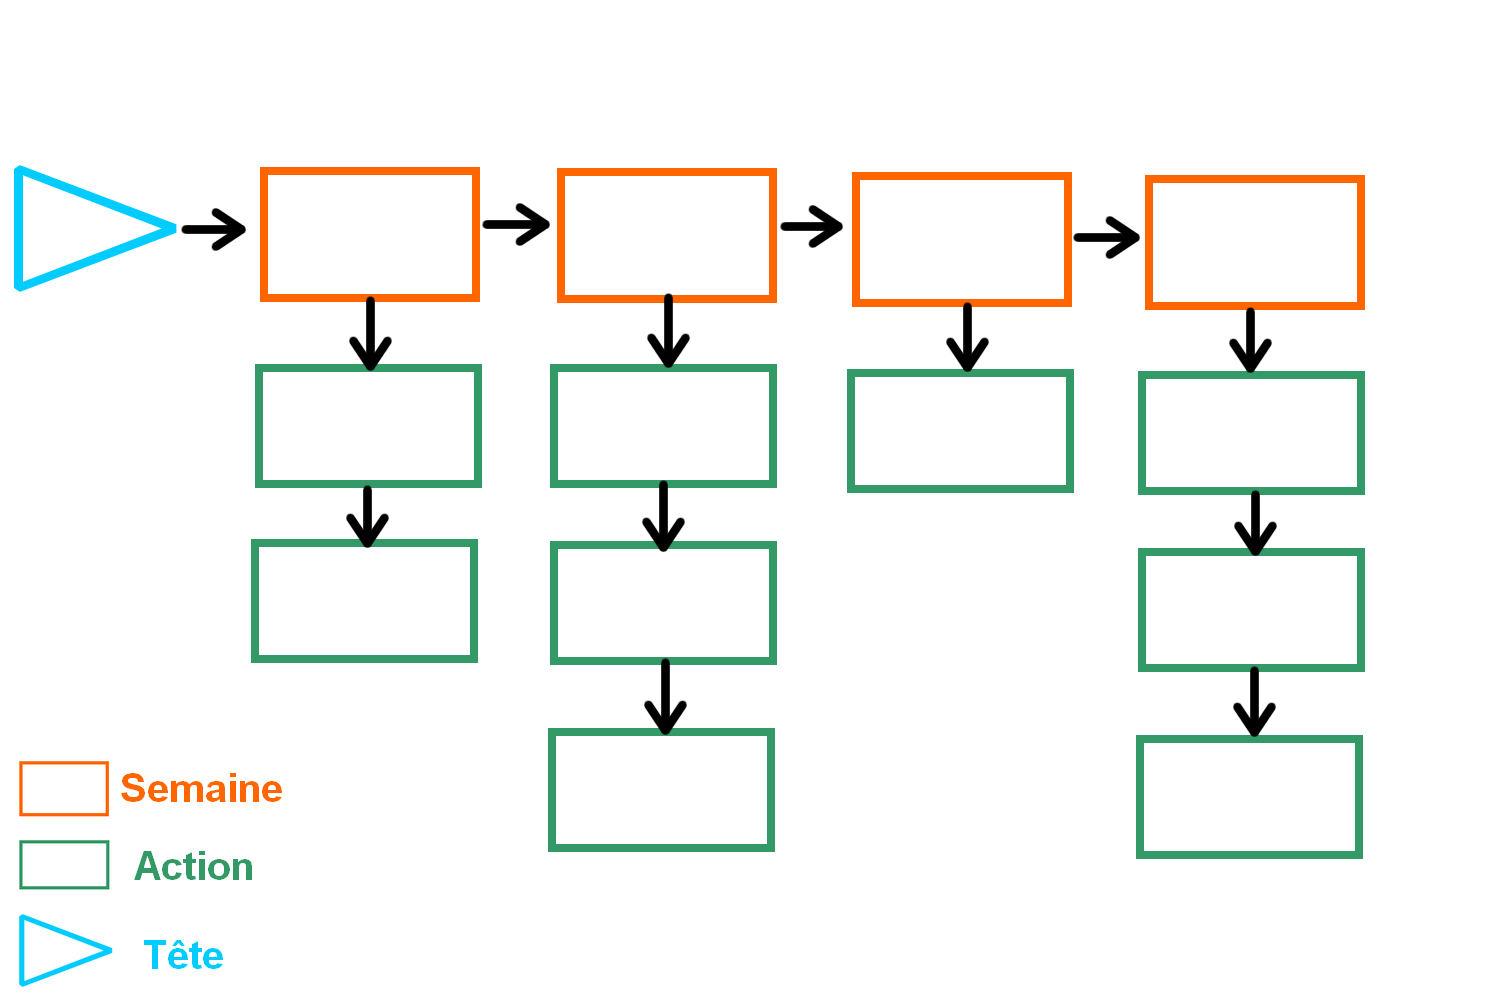
\includegraphics[scale=0.45]{structure.png}
	\centering
	\caption{Schéma de notre SDD "Agenda"}
\end{figure}



\subsection{Format des fichiers en entrée et en sortie}

Les formats des fichiers d'entrée et de sortie pour notre programme sont exactement les mêmes. Chaque ligne correspond à une activité et contient précisément dans cette ordre ces informations:

\begin{itemize}
	\item une année sur 4 bytes
	\item un numéro de semaine sur 2 bytes
	\item un chiffre compris entre $1$ et $7$ correspondant à un jour (lundi, mardi ...)
	\item une heure sur 2 bytes (08 pour 8h par exemple)
	\item Un nom pour l'activité noté précisément sur 10 bytes (on complète avec des espaces si besoin) \newline
\end{itemize}

Regardons maintenant un exemple de fichier d'entrée de notre programme et son fichier de sortie correspondant.\newline

\begin{figure}[H]
	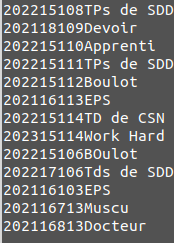
\includegraphics[scale=0.6]{entree.png}
	\centering
	\caption{Notre fichier d'entrée}
\end{figure}

Comme dit avant les informations sont bien notées dans le bon ordre. Une chose tout de même à remarquer ici: dans cette exemple nous avons fait exprès de glisser une erreur dans la ligne \textbf{"Docteur"}: en effet le chiffre des jours qui est censé être compris entre $1$ et $7$ vaut ici $8$ ! 

Regardons maintenant les fichiers de sortie obtenu:

\begin{figure}[H]
	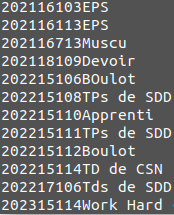
\includegraphics[scale=0.6]{sortie.png}
	\centering
	\caption{Notre fichier de sortie}
\end{figure}

Après le passage dans notre programme les informations stockées dans notre fichier d'entrée on était triées par ordre croissant de leur date dans notre SDD ! Ainsi, à la sortie, toutes nos informations sont écrites dans l'ordre croissant dans notre fichier de sortie ! De plus on remarque que la valeur de \textbf{"Docteur"} étant mauvaise, notre programme ne l'a pas ajouté dans la SDD et ainsi elle n'est pas dans le fichier de sortie !.



\section{Présentation des Fonctions}
Passons maintenant à la présentation de toutes nos fonctions.\newline

Mais avant cela nous nous devons de faire une aparté: nous avons pris la décision dans ce TP, dans chaque structure contenant des chaines de caractère de rajouter le caractère \textbf{'\textbackslash0'} en fin de chaine. En effet ce caractère est un élément essentiel du langage C est nous n'avons pas voulu nous en séparer. Sinon nous aurions été obligé de recoder toutes les fonctions de \textbf{string.h}. Ainsi dans chaque structure les chaines de caractères sont sur un bit de plus afin de stocker ce dit caractère !

\subsection{tete.h et tete.c}

Le fichier \textbf{tete.h} possède la structure représentant notre tête fictive. Ainsi elle est seulement composée d'un pointeur pointant sur une structure de type "semaine".\newline

\begin{figure}[H]
	\begin{lstlisting}
		typedef struct tete{
			semaine * debut;
		} tete;
	\end{lstlisting}
	\caption{Structure "tete"}
\end{figure}

La seule fonction unique à la structure "tete" est \textbf{AlloueTete} qui comme son nom l'indique va allouer de la mémoire à notre tête fictive. La fonction prend en argument un pointeur indirect de type "tete" et renvoie 0 si tout va bien ou -1 si l'allocation a raté.

\subsection{semaine.h et semaine.c}

Passons à \textbf{semaine.h} qui contient la structure "semaine".


\begin{figure}[H]
	\begin{lstlisting}
		typedef struct semaine{
			char annee_semaine[7];
			struct action * liste_action;
			struct semaine * suivant;
		} semaine;
	\end{lstlisting}
	\caption{Structure "semaine"}
\end{figure}

Comme avec "tete", la seule fonction en lien avec cette structure est \textbf{AlloueSemaine"} qui a pour but d'allouer de la mémoire à un élément de type "semaine". Cette fonction prend en argument un pointeur indirect sur une structure de type semaine, une string contenant une année et une autre string avec un numéro de semaine. Elle va tout de même contrôler si jamais les informations qu'ont lui a donné en paramètre sont valides (numéro de semaine bien compris entre 1 et 53).  Elle renvoie 0 si tout c'est bien passé et -1 si l'allocation a raté ou les valeurs entrées sont mauvaises. L'année ainsi que le numéro de semaine sont concaténés dans le champs \textbf{annee\_semaine}, cela nous evitera des tests en trop dans de futurs fonctions.

\subsection{action.h et action.c}
Enfin notre dernière structure est la structure \textbf{"action"} dont voici la forme:

\begin{figure}[H]
	\begin{lstlisting}
		typedef struct action{
			char jour_heure[4];
			char nom[11];
			struct action * suivant;
		} action;
	\end{lstlisting}
	\caption{Structure "action"}
\end{figure}

La fonction en lien avec celle-ci est \textbf{AlloueAction} qui va allouer de la mémoire pour une case action. Elle prend en argument un pointeur indirect sur une action ainsi que 3 strings possédants respectivement, une valeur entre 1 et 7 pour le jour, une heure et un nom. La fonction va vérifier si le jour ainsi que l'heure sont valides ! Si tout c'est bien passé (allocation réussi et champs valides) la fonction renvoi 0 sinon elle renvoi -1.

\subsection{commun.h et commun.c}

Passons à toutes les fonctions ayant un impact sur toute notre SDD !

\subsubsection{Lecture et Ecriture dans les fichiers}

Commençons avec \textbf{les gestions d'entrée et sortie:}\newline

La fonction \textbf{"LectureFichier"} va tenter d'ouvrir le fichier en lien avec le nom qu'il reçoit en paramètre. Si cela est possible il va lire tout son contenu et stocker dans différentes strings les informations qu'il en tire. Une fois à la fin d'une ligne, on oublie pas d'enlever le caractère '$\backslash$n' afin de passer à la ligne suivante puis on appelle la fonction \textbf{AjoutStruct} en lui donnant toutes les informations que l'on vient de récupérer. Une fois cela fait, on ferme le fichier. La fonction renvoie 1 si la lecture c'est bien passé, 0 sinon.\newline

La fonction \textbf{"EcritureFichier"} va elle prendre en argument un nom de fichier et la tête fictive de notre SDD. Si on a pas de problème d'ouverture de fichier, on va parcourir entièrement notre SDD. C'est à dire semaine après semaine tout en parcourant toutes les actions de chaque semaine. Elle va, à chaque action, rajouter une ligne dans notre fichier avec les informations correspondant à celle-ci. On fait bien attention de rajouter un '$\backslash$n' à chaque fin de ligne sauf la dernière pour respecter le format standard de nos fichiers. Grâce à cela un fichier produit par notre programme pourra être bien évidemment mis ensuite en entrée !

\subsubsection{Gestion d'allocation}

Voyons maintenant toutes les fonctions utilisant des allocations ou des libérations de mémoire !\newline

La fonction \textbf{"CreationElement"} est une fonction outil qui prend en argument 5 strings avec toutes les informations possibles d'une activité (année, numéro de semaine, jour, heure, nom) ainsi qu'un pointeur indirect sur une semaine. Il va allouer en mémoire la semaine ainsi que l'action correspondant aux informations données et les relier entre eux ! 
La fonction renvoie 1 si tout s'est bien passé, 0 si une allocation a ratée et -1 si les 2 ont ratées !\newline

\begin{figure}[H]
	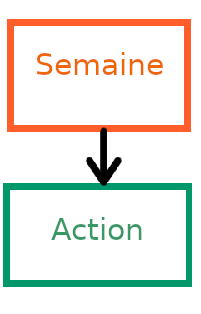
\includegraphics[scale=0.5]{nouvSemaine.png}
	\centering
	\caption{Représentation de l'élément crée}
	\label{element-default}
\end{figure}

La fonction \textbf{"LiberationElement"} fais l'inverse, elle libère un élément de la forme semaine pointant vers action. Le duo de ces des fonctions va nous faciliter la tâche lors de l'utilisation de la fonction \textbf{"SupprStruct"}.\newline

La fonction \textbf{"LibererStruct"} va entièrement libérer toute notre SDD. On lui donne simplement en argument notre tête fictive. Elle va parcourir l'intégralité de la SDD et libérer au fur et à mesure toutes les actions et les semaines. AU final on oublie pas de libérer la tête fictive !
 
 
\subsubsection{Ajout et Suppression}

On arrive aux deux fonctions les plus complexes.
Elles sont intégralement commentées dans notre fichier "commun.c" et nous allons brièvement les expliquer ici !\newline

La fonction \textbf{"AjoutStruct"} va être appelée par la fonction "LectureFichier" qui lui fourni toutes les informations sur une ligne de fichier ! Elle va ensuite crée un élément de la forme de la figure \ref{element-default}. Si on rencontre un problème lors de la création de cet élément, on le libère et on ne l'ajoute pas à la SDD !
Nous avons ensuite différents cas d'ajout à gérer:

\begin{itemize}
	\item L'ajout quand la SDD est vide : on fait simplement pointer notre tête fictive sur le nouvel élément.
	\item L'ajout quand la case semaine existe déjà ! A ce moment là, on doit vérifier si l'action que l'on souhaite ajouter ne doit pas être ajouté en tête de la liste des actions de cette semaines. Si c'est le cas on modifie le pointeur "liste\_action" de la dite semaine ! Sinon on fait un simple ajout avec les valeurs du pointeur précédent action ! On oublie pas de libérer la case semaine fraichement car une semblable existe déjà dans la SDD ! 
	\item L'ajout quand la semaine n'existe pas ! A ce moment là on doit vérifier que la semaine à ajouter n'est pas à positionner en tête de SDD, si c'est le cas on change le pointeur de notre tête fictive, sinon on ajoute simplement notre semaine avec le pointeur précédent semaine !\newline
\end{itemize}

La fonction \textbf{"SupprStruct"} prend elle en argument un pointeur sur notre tête fictive et sur un élément de la forme de la figure \ref{element-default} (c'est à dire une semaine pointant sur une action). On va parcourir toute notre SDD en cherchant une semaine puis une action identique à celle prise en argument ! Une fois cela fait, si on cette action existe, on la supprime, sinon on fait rien ! Si l'action est bien supprimée on renvoie 1, si la semaine visée n'existe pas dans la SDD on renvoie 0 enfin si l'action n'existe pas on renvoie -1.  Nous avons encore une fois plusieurs cas à traiter:

\begin{itemize}
	\item La semaine n'existe pas: on ne fait rien
	\item L'action n'existe pas: on ne fait rien
	\item On supprime la première action d'une semaine. A ce moment là on doit changer l'action pointée par la semaine puis libérer la mémoire de cette action.
	\item On supprime une action pas en tête. A ce moment là on a juste à changer les pointeurs en faisant pointer le précédents de cette dite action sur la suivant de celle-ci puis de libérer la mémoire de cette action !
	\item Après suppression d'une action, on se rend compte que la semaine est maintenant vide ! On doit donc la supprimer elle aussi ! Soit c'est la première et on change le pointeur de la tête fictive soit on joue rediriger le pointeur précédent. Dans tous les cas on oublie pas de libérer la semaine à supprimer !\newline
\end{itemize}

\subsubsection{Affichage}

La fonction \textbf{AffichageAgenda} est toute simple. Elle parcourt entièrement notre SDD et affiche pour chaque élément "semaine" toutes les actions qu'il contient ! On utilise un tableau statique contenant tous les jours de la semaine pour faire un affichage plus propre. Le principe est simple: On récupère la valeur ascii du jour à afficher auquel on enlève la valeur ascii du char "1". Ainsi, pour Lundi on aura l'indice 0, mardi l'indice 1 ... On a plus qu'à afficher la string présente à l'indice du tableau voulu !  

\subsection{contigue.h et contigue.c}

Enfin voyons les fonctions en lien avec la liste contiguë qui cherche un motif. Nous rappelons que l'on doit, à l'aide d'un motif pris en argument, chercher si celui-ci apparait dans le nom de nos actions et si c'est le cas, stocker la date de cette actions dans une liste contiguë.\newline
La liste contiguë est toutes simples: c'est un tableau de char en 2 dimensions statique ayant un nombre de ligne limité défini par la valeur \textbf{MAX\_TAILLE\_CONTIGUE} présent dans contigue.h. Chaque string contenu dans cette liste est de taille \textbf{TAILLE\_DATE\_ACTION}. Cette taille est de 10 car l'on stocke les 6 bytes de l'année ainsi que du numéro de semaine puis les 3 bytes du jour et de l'heure et enfin le char '$\backslash$0'. Nous avons mis la liste contiguë en variable globale dans le fichier contigue.h. Ainsi on commence à définir deux pointeurs de type "char", un de début et un de fin et on appelle la fonction InitContigue qui va les placer correctement.\newline

La fonction \textbf{InitContigue} prend donc en argument notre liste contiguë et deux pointeurs indirects "debut\_contigue" et "fin\_contigue". Au départ la liste étant vide, on les place tous les deux au début de la liste c'est à dire qu'ils prennent l'adresse "contigue[0]". Après cela on utilisera plus la notation "[ ]" des tableaux en C mais bien juste nos 2 pointeurs de début et de fin.

Ensuite, la fonction \textbf{RemplisContigue} prend en argument un motif, notre tête fictive et nos pointeurs de début et de fin. On va créer un pointeur "parcours\_contigue" qui aura pour but de parcourir la liste contiguë et un pointeur "dernier\_element" qui pointe sur la dernière position possible où écrire dans notre liste contiguë. Si on essaye d'écrire plus loin on n'écrit plus dans la zone fixe allouée à notre liste. C'est donc pour cela que l'on vérifie dans le if si on a dépassé cette valeur ou pas ! On a donc maintenant plus qu'à parcourir entièrement toutes notre SDD et vérifier si le motif apparait dans le nom des actions (et que la liste contiguë n'est pas pleine), si c'est le cas alors on ajoute les informations de date dans la liste.
La fonction va ensuite en toute fin placer le pointeur de fin de la liste contiguë qui correspond à l'adresse où se trouve la dernière chaine de caractère de taille 10.\newline

Au final \textbf{AfficheContigue} parcours tous les éléments existants dans la liste contiguë jusqu'à arriver au pointeur fin. On a utilisé une boucle for pour respecter les bonnes normes de code. Étant donné qu'on connait la taille de notre liste on passe par une boucle for ! On utilise le même tableau "tab\_jour" que dans "AfficheStruct" pour afficher plus proprement les jours de la semaine.


\section{Liste des cas}

Nous allons ici vous présenter la liste des cas possibles et leurs jeux de donnée attitrés afin que vous puissiez tous les tester.

\subsection{Lecture}
\subsection{Ajout}
\subsection{Suppression}
\subsection{Contiguë}

\section{Annexe}
\listoffigures



\end{document}
